\documentclass[aspectratio=169]{beamer}
\mode<presentation>
%\usetheme{Warsaw}
%\usetheme{Goettingen}
\usetheme{Hannover}
%\useoutertheme{default}

%\useoutertheme{infolines}
\useoutertheme{sidebar}
\usecolortheme{dolphin}


\setbeamersize{sidebar width left=0pt} % to remove the sidebar
\beamertemplatenavigationsymbolsempty % To remove the navigation symbols on the bottom right.
\setbeamersize{text margin left=10mm,text margin right=10mm} % Specify margins

\usepackage{amsmath}
\usepackage{amssymb}
\usepackage{listings}
\usepackage{enumerate}
\usepackage{animate}
\usepackage{hyperref}
\hypersetup{
    colorlinks=true,
    linkcolor=blue,
    filecolor=magenta,      
    urlcolor=cyan,
}

%%%%For drawing graphs
% a nice font
\usepackage{kpfonts}

% basic text stuff
\usepackage[utf8]{inputenc}
\usepackage[T1]{fontenc}

\usepackage{tikz} % main tikz package
\usepackage{tikz-network} % for network / graph utilities

% for a nicer colorscheme
%\input{colors.tex} % By nemo.fournier https://nemo.kiwi/latex.html#h3_colors
%%%%%%%%%%%%%%%%%%%%%%%%%%%%%%%

\begin{document}
 
\urlstyle{same}

%some bold math symbosl
\newcommand{\Cov}{\mathrm{Cov}}
\newcommand{\Var}{\mathrm{Var}}
\newcommand{\brho}{\boldsymbol{\rho}}
\newcommand{\bSigma}{\boldsymbol{\Sigma}}
\newcommand{\btheta}{\boldsymbol{\theta}}
\newcommand{\bbeta}{\boldsymbol{\beta}}
\newcommand{\bmu}{\boldsymbol{\mu}}
\newcommand{\bW}{\mathbf{W}}
\newcommand{\one}{\mathbf{1}}
\newcommand{\bH}{\mathbf{H}}
\newcommand{\by}{\mathbf{y}}
\newcommand{\bolde}{\mathbf{e}}
\newcommand{\bx}{\mathbf{x}}

\newcommand{\cpp}[1]{\texttt{#1}}

%--------------------------------------------------
\providecommand{\abs}[1]{\lvert#1\rvert}
\providecommand{\norm}[1]{\lVert#1\rVert}
\providecommand{\Blue}[1]{\textcolor{blue}{#1}}
\providecommand{\Red}[1]{\textcolor{red}{#1}}  
\providecommand{\Purple}[1]{\textcolor{purple}{#1}} %for notations
\newcommand{\celsius}{\ensuremath{^\circ}C}
\newcommand\thfore{\mathord{\therefore}\,}
%------------------------------------------------------------------

\title{Lecture 4. Graph Coloring Problem}
%\author{\includegraphics[width=.8\textwidth,height=.7\textheight]{lecture1-fig0.jpg}}

\date{ }
%------------------------------------------------------------------

\frame[plain]{\titlepage}

\begin{frame}[plain]{} 


\begin{center}
  {\bf Given a set of $k$ colors, can we assign colors to each vertex
     so that no two neighbors are assigned the same color?
  }
\end{center}

{\small  We may revise the question as 
``Given a graph, what is \Red{the minimum number of colors} 
that can be assigned to each vertex so that no two neighbors have the same color?"
}

\begin{columns}[t] % contents are top vertically aligned
\begin{column}[c]{5cm}

%%%Sample code for drawing is after \end{document}
  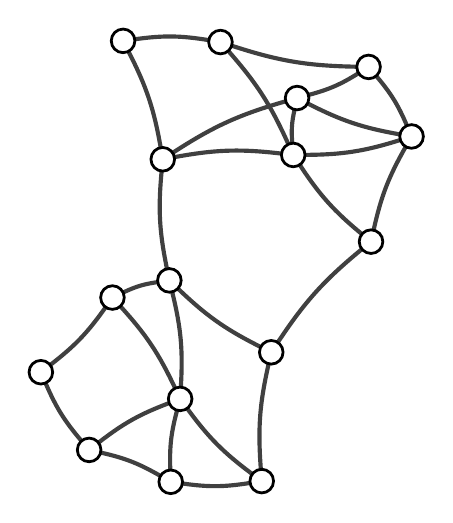
\begin{tikzpicture}[>=stealth']
 %   \coordinate (13) at (3.572,1.845);
    
    \Vertex[color=white,x=3.9,y=5.074,size=0.3,]{0}
    \Vertex[color=white,x=3.851,y=4.351,size=0.3,]{1}
    \Vertex[color=white,x=5.354,y=4.586,size=0.3,]{2}
    \Vertex[color=white,x=4.839,y=3.250,size=0.3,]{3}
    \Vertex[color=white,x=2.927,y=5.785,size=0.3, ]{4}
    \Vertex[color=white,x=1.690,y=5.800,size=0.3, ]{5}    
    \Vertex[color=white,x=2.194,y=4.296,size=0.3,]{6} 
    \Vertex[color=white,x=4.808,y=5.469,size=0.3,]{7}
    \Vertex[color=white,x=0.646,y=1.592,size=0.3,]{8}
    \Vertex[color=white,x=2.415,y=1.253,size=0.3,]{9}
    \Vertex[x=2.295,y=0.200,size=0.3, color=white,]{10}
    \Vertex[color=white,x=1.259,y=0.605,size=0.3,]{11}
    \Vertex[color=white,x=2.278,y=2.758,size=0.3,]{12}
    \Vertex[color=white,x=3.572,y=1.845,size=0.3,]{13}
    \Vertex[color=white,x=1.555,y=2.540,size=0.3,]{14}
    \Vertex[color=white,x=3.451,y=0.209,size=0.3,]{15}
        
    \Edge[,bend=-8.531](0)(1)
    \Edge[,bend=-8.531](0)(2)
    \Edge[,bend=-8.531](0)(6)
    \Edge[,bend=-8.531](0)(7)
    \Edge[,bend=-8.531](1)(2)
    \Edge[,bend=-8.531](1)(3)
    \Edge[,bend=-8.531](1)(4)
    \Edge[,bend=-8.531](1)(6)
    \Edge[,bend=-8.531](2)(3)
    \Edge[,bend=-8.531](2)(7)
    \Edge[,bend=-8.531](3)(13)
    \Edge[,bend=-8.531](4)(5)
    \Edge[,bend=8.531](5)(6)    
    \Edge[,bend=-8.531](4)(7)
    \Edge[,bend=-8.531](6)(12)
    \Edge[,bend=-8.531](8)(11)
    \Edge[,bend=-8.531](8)(14)
    \Edge[,bend=-8.531](9)(10)
    \Edge[,bend=-8.531](9)(12)
    \Edge[,bend=-8.531](9)(14)
    \Edge[,bend=-8.531](9)(15)
    \Edge[,bend=-8.531](10)(11)
    \Edge[,bend=-8.531](9)(11)
    \Edge[,bend=-8.531](10)(15)
    \Edge[,bend=-8.531](12)(13)
    \Edge[,bend=-8.531](12)(14)
    \Edge[,bend=-8.531](13)(15)
    
   \end{tikzpicture}    
   
  \end{column} \pause
  \begin{column}[c]{5cm}
     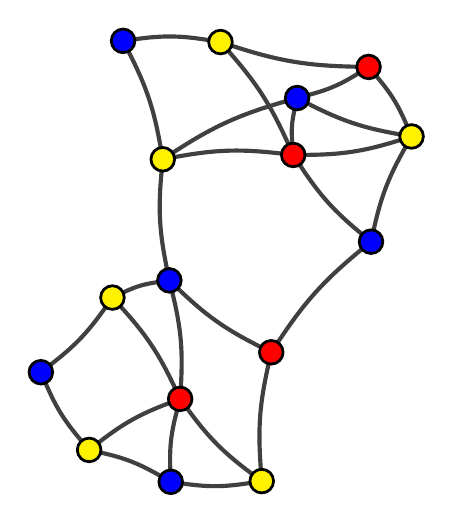
\begin{tikzpicture}[>=stealth']
 %   \coordinate (13) at (3.572,1.845);
 
    \Vertex[color=blue,x=3.9,y=5.074,size=0.3,]{0}
    \Vertex[color=red,x=3.851,y=4.351,size=0.3,]{1}
    \Vertex[color=yellow,x=5.354,y=4.586,size=0.3,]{2}
    \Vertex[color=blue,x=4.839,y=3.250,size=0.3,]{3}
    \Vertex[color=yellow,x=2.927,y=5.785,size=0.3, ]{4}
    \Vertex[color=blue,x=1.690,y=5.800,size=0.3, ]{5}    
    \Vertex[color=yellow,x=2.194,y=4.296,size=0.3,]{6} 
    \Vertex[color=red,x=4.808,y=5.469,size=0.3,]{7}
    \Vertex[color=blue,x=0.646,y=1.592,size=0.3,]{8}
    \Vertex[color=red,x=2.415,y=1.253,size=0.3,]{9}
    \Vertex[color=blue,x=2.295,y=0.200,size=0.3,]{10}
    \Vertex[color=yellow,x=1.259,y=0.605,size=0.3,]{11}
    \Vertex[color=blue,x=2.278,y=2.758,size=0.3,]{12}
    \Vertex[color=red,x=3.572,y=1.845,size=0.3,]{13}
    \Vertex[color=yellow,x=1.555,y=2.540,size=0.3,]{14}
    \Vertex[color=yellow,x=3.451,y=0.209,size=0.3,]{15}
    
    \Edge[,bend=-8.531](0)(1)
    \Edge[,bend=-8.531](0)(2)
    \Edge[,bend=-8.531](0)(6)
    \Edge[,bend=-8.531](0)(7)
    \Edge[,bend=-8.531](1)(2)
    \Edge[,bend=-8.531](1)(3)
    \Edge[,bend=-8.531](1)(4)
    \Edge[,bend=-8.531](1)(6)
    \Edge[,bend=-8.531](2)(3)
    \Edge[,bend=-8.531](2)(7)
    \Edge[,bend=-8.531](3)(13)
    \Edge[,bend=-8.531](4)(5)
    \Edge[,bend=8.531](5)(6)    
    \Edge[,bend=-8.531](4)(7)
    \Edge[,bend=-8.531](6)(12)
    \Edge[,bend=-8.531](8)(11)
    \Edge[,bend=-8.531](8)(14)
    \Edge[,bend=-8.531](9)(10)
    \Edge[,bend=-8.531](9)(12)
    \Edge[,bend=-8.531](9)(14)
    \Edge[,bend=-8.531](9)(15)
    \Edge[,bend=-8.531](10)(11)
    \Edge[,bend=-8.531](9)(11)
    \Edge[,bend=-8.531](10)(15)
    \Edge[,bend=-8.531](12)(13)
    \Edge[,bend=-8.531](12)(14)
    \Edge[,bend=-8.531](13)(15)
    
   \end{tikzpicture}    
  \end{column}
  \end{columns}

    
\end{frame}

\begin{frame}[plain]{}

 {\bf Definition 4.1.} The \Blue{chromatic number} of a graph is 
 the minimum number of colors needed for a coloring of the graph. 
 The chromatic number of a graph $G$ is denoted by \Blue{$\chi(G)$}. \pause 
 \medskip
 
  {\bf Example 4.2.} What are the chromatic numbers of the graphs $G$ and $H$?
  \begin{center}
         \includegraphics[height=3.8cm]{./img/lecture4-fig1.png}
       \end{center}
 \vspace{.5in} 
 
\end{frame}

\begin{frame}[plain]{}

 Answer:
 
 \begin{center}
         \includegraphics[height=3.8cm]{./img/lecture4-fig2.png}
       \end{center}
 
\end{frame}


\begin{frame}[plain]{}


 A \Blue{complete graph on $n$ vertices}, denoted by \Blue{$K_n$}, 
 is a \emph{simple graph} that contains exactly one edge between each pair of distinct vertices
 
 \begin{center}
         \includegraphics[height=3cm]{./img/lecture4-fig3.png}
       \end{center}


{\bf Example 4.3.} What is $\chi(K_n)$? %Rosen, sec 10.8, p730,  Example 2
\vspace{.5in}

\end{frame}

\iffalse %%%%%%%%%%%%%%%%%%%%%%%%%%%%%%%%%%%%%%%
\begin{frame}[plain]{TO DO: Make animation}
 
  A \Blue{bipartite graph} (also called a \Blue{bigraph})
   is a graph whose vertices can be partitioned into two
   parts, say $\{v_1, v_2,..., v_n\}$ and $\{w_1, w_2,..., w_m\}$
    so that all edges join some $v_i$ to some $w_j$;
    no two vertices $v_i$ and $v_j$ are adjacent, 
    nor are any vertices $w_i$ and $w_j$.~\footnote{That is,
    vertices are decomposed into two disjoint subsets 
    such that no two vertices within the same subset are adjacent.}
     
 \vspace{.5in}
   Use 'lecture2-bipartite.gif' to animation here
  %https://medium.com/python-in-plain-english/bipartite-graphs-a-fundamental-concept-in-graph-theory-779ddf45218d
 \begin{center}
   \animategraphics[loop, autoplay, controls, width=\textwidth]{10}{./img/lecture4-bipartite-}{0}{16}
       \end{center}
       
 \end{frame}
\fi %%%%%%%%%%%%%%%%%%%%%%%

\begin{frame}[plain]{}
 
  A \Blue{bipartite graph} (also called a \Blue{bigraph})
   is a graph whose vertices can be partitioned into two
   parts, say $\{v_1, v_2,..., v_n\}$ and $\{w_1, w_2,..., w_m\}$
    so that all edges join some $v_i$ to some $w_j$;
    no two vertices $v_i$ and $v_j$ are adjacent, 
    nor are any vertices $w_i$ and $w_j$.~\footnote{That is,
    vertices are decomposed into two disjoint subsets 
    such that no two vertices within the same subset are adjacent.}
     
    \begin{center}
         \includegraphics[height=1.8cm]{./img/lecture4-fig4.png}
       \end{center}
       \pause
       
  {\bf Example 4.4.} Remove 4 edges from the complete graph $K_5$ to
     to  make a bipartite graph.
 
  \begin{center}
    \includegraphics[height=2.8cm]{./img/lecture4-fig5.png}
  \end{center}
   %https://www2.math.binghamton.edu/lib/exe/fetch.php/people/grads/eppolito/graph_theory_quiz_solutions.pdf
   %Exam1F22-makeup
   
  
 \end{frame}
 
 
 
 \begin{frame}[plain]{}
 
  A \Blue{complete bipartite graph $\mathbf{K_{m,n}}$} is
  a special kind of bipartite graph where every vertex of the first subset
  of $m$ vertices is connected 
  to every vertex of the second subset of $n$ vertices.  
  \begin{center}
         \includegraphics[height=3.5cm]{./img/lecture4-fig6.png}
       \end{center}
  
 {\bf Example 4.5} What is $\chi(K_{m,n})$? %Rosen, sec 10.8, p730,  Example 3
\vspace{.3in}

\end{frame}

\begin{frame}[plain]{}

  {\bf Example 4.6 (Scheduling).}
   A college registra would like to schedule the following courses in 
    as few time slots as possible: {\bf Physics}, {\bf Computer Science}, 
      {\bf Chemistry}, {\bf Calculus}, {\bf Discrete Math}, {\bf Biology},
      and {\bf Psychology}. However, from previous experience, the following
      pairs of classes always have students in common, so they can't be scheduled
      in the same time slot:
      \medskip
      
      \begin{center}
      \begin{tabular}{|c|l|} \hline
       Physics  & Computer Science, Chemistry \\ \hline
       Calculus & Chemistry, Physics, Compute Science, \\ 
                &  Discrete Math, Biology \\ \hline
       Discrete math & computer Science, Biology \\ \hline
       Psychology & Biology, Chemistry \\ \hline
      \end{tabular}
      \end{center}
      
    What is the \Red{fewest} number of time slots needed to schedule all these classes without conflicts? 
 
\end{frame}

\begin{frame}[plain]{}

 \begin{itemize}
  \item The natural way to model this problem with a graph is to make each course into
     a vertex and connect any two vertices (representing courses) that cannot be scheduled 
     in the same time slot: \pause 
      \begin{center}
         \includegraphics[height=3cm]{./img/lecture4-fig7.png}
       \end{center}\pause 
    \item Then,  what is the \Red{fewest} number of time slots needed to schedule all these classes without conflicts? 
     That is, how many colors are needed for the graph coloring?
    \item  The minimum number of colors for the graph coloring is the fewest number of time slots needed for the courses. 
 \end{itemize} 
\end{frame}


\begin{frame}[plain]{}
 
 
 {\bf Activity 4.7.} (Allocating the radio frequencies to the tower in a location)
  Suppose some of the transmitters are
  located so close  that they can overlap and there will be a disturbance.
 We need to allocate different frequencies to the
towers which are too close to each other in a location.
   How many different frequencies are needed for six transmitter towers
    located at the distances 
  shown in the table, if two towers cannot use the same frequency 
  when they are within 150 km of each other?
  
  \begin{center}
         \includegraphics[height=4.5cm]{./img/lecture4-fig8.png}
       \end{center}
  %Rosen, sec 10.8, p733,  #18

\end{frame}

%\begin{frame}[plain]{Sudoku}

%https://www.youtube.com/watch?v=LFKZLXVO-Dg&t=461s

%\end{frame}


\end{document}
%%%%%%%%%%%%%%%%%%%%%



""" 
 A graph is 2-colorable if and only if it does not contain an odd cycle.
 
 https://math.libretexts.org/Bookshelves/Combinatorics_and_Discrete_Mathematics/Applied_Combinatorics_(Keller_and_Trotter)/05%3A_Graph_Theory/5.04%3A_Graph_Coloring#:~:text=following%20theorem%20shows.-,Theorem%205.21,not%20contain%20an%20odd%20cycle.&text=Let%20G%3D(V%2CE,vertices%20between%20A%20and%20B.
""" 
 
 
 
%%Sample graph drawing
\begin{frame}[plain]{}


    \begin{tikzpicture}[>=stealth']
        %\clip (0,0) rectangle (6,6);
        \coordinate (13) at (3.572,1.845);
        \fill [orange, opacity=0.4] plot [smooth cycle, tension=1] coordinates {(13) ($ (13) + (-0.4,0.3)$) ($ (13) + (-0.5,0.1)$)};
        \fill [orange, opacity=0.4] plot [smooth cycle, tension=1] coordinates {(13) ($ (13) + (-0.2,-0.4)$) ($ (13) + (0.05,-0.4)$)};
        \fill [orange, opacity=0.4] plot [smooth cycle, tension=1] coordinates {(13) ($ (13) + (0.15,0.45)$) ($ (13) + (0.4,0.4)$)};

        \node (degree) at ($ (13) + (2.7,0.2) $)
        {\color{orange}{\tiny{\emph{node degree} (number
        of neighbours)}}};
        \node (degree) at ($ (13) + (3,-0.2) $)
        {\color{orange}{\tiny{\emph{node strength} (sum of adjacent edges
        weights)}}};

        \Vertex[color=brokenwhite!30,x=3.9,y=5.074,size=0.3,]{0}
        \Vertex[color=brokenwhite!30,x=3.851,y=4.351,size=0.3,]{1}
        \Vertex[color=brokenwhite!30,x=5.354,y=4.586,size=0.3,]{2}
        \Vertex[color=green, x=4.839,y=3.250,size=0.3,]{3}
        \node (clustering) at (6.4,3.25) {\color{green}{\tiny{\shortstack{\emph{clustering coefficient}\\ fraction of triangles in \\ the node's neighbourhood}}}};
        \Vertex[color=blue!50, x=2.927,y=5.785,size=0.3, ]{4}
        \Vertex[x=1.690,y=5.800,size=0.3,color = blue!50, ]{5}
        \node (shortest) at (3.2,3.4) {\color{blue}{\tiny{\emph{shortest paths}}}};
        \Vertex[x=2.194,y=4.296,size=0.3,color = blue]{6}
        \node (centrality) at (-0.1, 4.3)
        {\color{blue}{\tiny{\shortstack{\emph{betweenness centrality}\\
        fraction of all pairwise shortest \\ paths going through a node}}}};
        \Vertex[color=brokenwhite!30,x=4.808,y=5.469,size=0.3,]{7}
        \Vertex[color=brokenwhite!30,x=0.646,y=1.592,size=0.3,]{8}
        \Vertex[color=brokenwhite!30,x=2.415,y=1.253,size=0.3,]{9}
        \Vertex[x=2.295,y=0.200,size=0.3, color = blue!50,]{10}
        \Vertex[color=blue!50,x=1.259,y=0.605,size=0.3,]{11}
        \Vertex[color=brokenwhite!30,x=2.278,y=2.758,size=0.3,]{12}
        \Vertex[color=orange,x=3.572,y=1.845,size=0.3,]{13}
        \Vertex[color=brokenwhite!30,x=1.555,y=2.540,size=0.3,]{14}
        \Vertex[color=brokenwhite!30,x=3.451,y=0.209,size=0.3,]{15}
        \Edge[,bend=-8.531](0)(1)
        \Edge[,bend=-8.531](0)(2)
        %\Edge[,bend=-8.531](0)(5)
        \Edge[,bend=-8.531](0)(6)
        \Edge[,bend=-8.531](0)(7)
        \Edge[color=green,bend=-8.531](1)(2)
        \Edge[color=green,bend=-8.531](1)(3)
        \Edge[,bend=-8.531](1)(4)
        \Edge[,bend=-8.531](1)(6)
        \Edge[color=green,bend=-8.531](2)(3)
        \Edge[,bend=-8.531](2)(7)
        \Edge[,bend=-8.531](3)(13)
        \Edge[,bend=-8.531](4)(5)
        \Edge[lw=2, color=blue!50 ,bend=8.531](5)(6)
        \Edge[,bend=-8.531](4)(7)
        \Edge[lw=2, color=blue!50, style={dashed},bend=-8.531](4)(6)
        \Edge[lw=2, color=blue!50 ,bend=-8.531](6)(12)
        \Edge[lw=2, color=blue!50, style={dashed},bend=-8.531](6)(14)
        %\Edge[,bend=-8.531](8)(10)
        \Edge[,bend=-8.531](8)(11)
        %\Edge[,bend=-8.531](8)(12)
        \Edge[,bend=-8.531](8)(14)
        \Edge[lw=2, color=blue!50,bend=-8.531](9)(10)
        \Edge[lw=2, color=blue!50 ,bend=-8.531](9)(12)
        \Edge[,bend=-8.531](9)(14)
        \Edge[,bend=-8.531](9)(15)
        \Edge[,bend=-8.531](10)(11)
        \Edge[,bend=-8.531](9)(11)
        \Edge[lw=2, color=blue!50, style={dashed},bend=-8.531](11)(14)
        \Edge[,bend=-8.531](10)(15)
        \Edge[,bend=-8.531](12)(13)
        \Edge[,bend=-8.531](12)(14)
        %\Edge[,bend=-8.531](13)(14)
        \Edge[,bend=-8.531](13)(15)
   \end{tikzpicture}
   
 \end{frame}

